% cuADMM reorganization plan -- self-contained LaTeX source (pdflatex, two runs for references).
\documentclass[11pt]{article}
\PassOptionsToPackage{obeyspaces,spaces}{url}

\usepackage[T1]{fontenc}
\usepackage[utf8]{inputenc}
\usepackage{lmodern}
\usepackage[margin=1in]{geometry}
\usepackage{microtype}
\usepackage{amsmath,amssymb,mathtools}
\usepackage{booktabs,tabularx,longtable,array}
\usepackage{enumitem}
\usepackage[dvipsnames]{xcolor}
\usepackage{listings}
\usepackage{tikz}
\usetikzlibrary{positioning,arrows.meta,shapes.geometric,fit}
\usepackage{caption}
\usepackage{tcolorbox}
\usepackage[colorlinks=true,linkcolor=NavyBlue,citecolor=ForestGreen,urlcolor=NavyBlue]{hyperref}
\usepackage{xurl}

% ---------------------------------------------------------------- macros
\DeclareUrlCommand\code{\urlstyle{tt}}
\Urlmuskip=0mu\relax
\newcommand{\R}{\mathbb{R}}
\newcommand{\Sym}{\mathbb{S}}
\newcommand{\K}{\mathcal{K}}
\newcommand{\Kd}{\mathcal{K}^{*}}
\newcommand{\A}{\mathcal{A}}
\newcommand{\Ad}{\mathcal{A}^{*}}
\newcommand{\Proj}{\Pi}
\newcommand{\inner}[2]{\langle #1, #2\rangle}
\newcommand{\norm}[1]{\lVert #1\rVert}
\newcommand{\svec}{\operatorname{svec}}

\setlist{itemsep=2pt,topsep=4pt}
\setlength{\parskip}{3pt}

\lstdefinestyle{cpp}{
  language=C++,
  basicstyle=\ttfamily\footnotesize,
  keywordstyle=\color{NavyBlue}\bfseries,
  commentstyle=\color{Gray}\itshape,
  stringstyle=\color{BrickRed},
  breaklines=true,
  columns=fullflexible,
  keepspaces=true,
  frame=single,
  rulecolor=\color{Gray!50},
  xleftmargin=4pt,
  xrightmargin=4pt,
  aboveskip=6pt,
  belowskip=6pt,
  showstringspaces=false
}
\lstdefinestyle{plain}{
  language={},
  basicstyle=\ttfamily\footnotesize,
  columns=fullflexible,
  keepspaces=true,
  frame=single,
  rulecolor=\color{Gray!50},
  breaklines=true
}
\lstset{style=cpp}

\newtcolorbox{decision}[1]{colback=NavyBlue!4,colframe=NavyBlue!60,fonttitle=\bfseries,title={#1},boxrule=0.6pt,arc=2pt,left=4pt,right=4pt,top=3pt,bottom=3pt}
\newtcolorbox{warnbox}[1]{colback=BrickRed!4,colframe=BrickRed!60,fonttitle=\bfseries,title={#1},boxrule=0.6pt,arc=2pt,left=4pt,right=4pt,top=3pt,bottom=3pt}

\title{\textbf{Reorganizing cuADMM}\\[4pt]
\large An ADMM-first, cone-extensible architecture with pluggable PSD-projection strategies\\ and cuDSS / CHOLMOD linear-system backends}
\author{Reorganization plan for the cuADMM developers}
\date{October 13, 2026\\[2pt]
\small Baseline: \code{main} at \code{9bb4ba5} (submodule \code{psd_projection} at \code{b566590}),\\
\small plus the uncommitted penalty-rule edit of October 13, 2026 (Section~\ref{sec:penalty})}

\begin{document}
\maketitle

\begin{abstract}
cuADMM is a GPU solver for large multi-block conic programs, built around the first-order method of
\cite{cuadmm} and the factorization-free PSD projection of \cite{composite}. Its numerics are sound and
well tested, but nearly all logic lives in one class (\code{SDPSolver}) whose \code{solve()} method spans
about 1{,}080 lines, configuration is spread over positional arguments, public fields and preprocessor
constants, and several algorithmic options are either compiled out or unreachable. This document is a
complete plan to reorganize the code into a layered library in which (i) plain ADMM with step length
$\tau\in(0,2)$ is the default algorithm and sGS-ADMM is a runtime option, justified by the
equivalence result of \cite{afterimage}; (ii) every cone is a plug-in behind one interface, so that
second-order and other cones can be added without touching the solver; (iii) the PSD projection is a
catalog of explicit, named strategies---including the composite polynomial filter of \cite{composite},
integrated directly instead of through a submodule---selected by a documented policy; and (iv) the
normal-equation solve is an interface with a cuDSS backend first and a CHOLMOD backend second. The plan
lists the defects found during the review, the target architecture with interface sketches and naming
conventions, a single table of options and defaults, a test strategy, and an incremental migration in
ten phases, each with acceptance criteria.
\end{abstract}

\tableofcontents


%=======================================================================================================
\section{Summary}\label{sec:summary}

\paragraph{Decisions already taken.}
\begin{enumerate}[label=\textbf{D\arabic*.}]
  \item \textbf{ADMM is the default algorithm.} The default iteration is plain (two-block) ADMM with
  multiplier step length $\tau = 1.618$; $\tau = 1.918$ is offered as the aggressive preset, and any
  $\tau\in(0,2)$ is accepted. sGS-ADMM becomes a \emph{runtime} option (today it is removed at compile
  time by \code{CUADMM_PLAIN_ADMM_ONLY}). Rationale: ADMM and sGS-ADMM share the same fixed-point map
  in the $z$-variable, and every $\tau\in(0,2)$ is admissible \cite{afterimage,gabay,chen2021}
  (Section~\ref{sec:math-admm}).
  \item \textbf{Linear systems: cuDSS first, CHOLMOD second.} The normal-equation solver is an
  interface with two production backends: cuDSS (GPU factorization and GPU solves, preferred when
  available) and CHOLMOD (CPU factorization, CPU or dense-GPU solves, always available). A dense
  cuSOLVER backend is optional (Section~\ref{sec:linsys}).
  \item \textbf{Composite polynomial filtering is integrated directly.} The kernels of
  \cite{composite} move into cuADMM as one PSD projection strategy among several; the
  \code{psd_projection} submodule is retired (Section~\ref{sec:psd}).
  \item \textbf{Cones are plug-ins.} Free, nonnegative and PSD blocks are ported to a common
  \code{Cone} interface; second-order cones are the first new cone (Section~\ref{sec:cones}).
  \item \textbf{Software-engineering standards.} One options object with one table of defaults, explicit
  ownership of GPU resources, no allocation inside the iteration loop, deterministic by default,
  consistent naming, and a behavior-preserving migration in which every structural step reproduces the
  current iterates bit for bit (Sections~\ref{sec:principles}--\ref{sec:migration}).
\end{enumerate}

\paragraph{What the reader should take away.}
Table~\ref{tab:phases-short} summarizes the migration. Phases 0--6 restructure the code without changing
its iterates (except for explicit bug fixes); Phases 7--9 change behavior on purpose and are validated
against tolerances instead of bitwise histories.

\begin{table}[h]
\centering\small
\begin{tabularx}{\textwidth}{@{}l>{\raggedright\arraybackslash}X l@{}}
\toprule
Phase & Content & Iterates \\
\midrule
0 & Safety net: frozen baseline histories, CI build matrix, environment fixes & unchanged \\
1 & Cleanup: dead code, compile-time algorithm flag, the defects of Table~\ref{tab:defects} that are one-line fixes & unchanged$^{\dagger}$ \\
2 & \code{SolverOptions}: one source of defaults; CLI and MATLAB rebuilt on it & unchanged \\
3 & Core infrastructure: \code{GpuContext}, stream pool, workspace arena & unchanged \\
4 & Algorithm layer: \code{IterationScheme}, \code{PenaltyPolicy}, termination, observers & unchanged \\
5 & Cone layer: \code{Cone} interface; free, nonnegative and PSD cones ported & unchanged \\
6 & PSD strategies and composite filter integrated; submodule retired & unchanged$^{\ddagger}$ \\
7 & Linear systems: \code{NormalEquationSolver}, CHOLMOD port, cuDSS backend, presolve & within tolerance \\
8 & Data layout: variables grouped by cone, concurrent cone projections & within tolerance \\
9 & New cones: second-order and rotated second-order & new tests \\
10 & Documentation, examples, benchmarks, release & --- \\
\bottomrule
\end{tabularx}
\caption{Migration phases (details in Section~\ref{sec:migration}). $^{\dagger}$Except the stream race
fix (B2), which only removes a possible nondeterminism. $^{\ddagger}$For the exact-EVD paths; the
composite path changes because of the math-mode fix (B1).}
\label{tab:phases-short}
\end{table}

%=======================================================================================================
\section{Background and the three papers}\label{sec:background}

\begin{itemize}
  \item \textbf{cuADMM} \cite{cuadmm} introduced the solver: sGS-ADMM for multi-block SDPs, PSD
  projection by cuSOLVER (batched Jacobi for many small blocks, QR-based EVD on streams for larger
  ones), and a hybrid CPU--GPU normal-equation solve with CHOLMOD, building on the trajectory
  optimization pipeline of \cite{wafr}. Its experiments target sparse moment relaxations of
  contact-rich planning and multi-block SDPs from Mittelmann's collection.
  \item \textbf{Composite polynomial filtering} \cite{composite} replaces the eigenvalue decomposition
  of a large dense block by a short composition of odd degree-5 polynomials evaluated with GEMMs in
  FP16 or FP32, after scaling the spectrum with a Lanczos bound. It is designed as a low-precision
  \emph{warm start} inside ADMM, followed by FP64 projections, and notes that ADMM quickly enters a
  low-rank regime \cite{kang2025local} in which LOBPCG becomes attractive.
  \item \textbf{Afterimage slow regions} \cite{afterimage} studies first-order methods for linear
  conic programs as fixed-point iterations. Its Table~1 and Appendix~A.2 show that ADMM and sGS-ADMM
  induce the \emph{same} fixed-point map in the auxiliary variable $z$, which is the basis of
  decision D1.
\end{itemize}

%=======================================================================================================
\section{Mathematical specification}\label{sec:math}

This section fixes the mathematics the code must implement; class and function names in later sections
refer to the symbols introduced here (Appendix~\ref{app:notation}).

\subsection{Problem class}
Let $\mathbb{X} = \mathbb{X}_1\times\cdots\times\mathbb{X}_B$ and
$\K = \K_1\times\cdots\times\K_B$ with each $\K_\beta$ a closed convex cone in $\mathbb{X}_\beta$.
cuADMM solves the primal--dual pair
\begin{equation}\label{eq:pd}
\min_{X\in\mathbb{X}}\ \inner{C}{X}\ \ \text{s.t.}\ \ \A X = b,\ X\in\K,
\qquad
\max_{y\in\R^m,\ S\in\mathbb{X}}\ \inner{b}{y}\ \ \text{s.t.}\ \ \Ad y + S = C,\ S\in\Kd .
\end{equation}
Today $\K_\beta\in\{\Sym^n_+,\ \R^n_+,\ \R^n\}$ (block codes \code{s}, \code{l}, \code{u}), with dual
cones $\Sym^n_+$, $\R^n_+$ and $\{0\}$. PSD blocks are stored in $\svec$ form (upper triangle, column by
column, off-diagonal entries multiplied by $\sqrt2$), so $\inner{\cdot}{\cdot}$ is the Euclidean inner
product on the stacked vector.

\subsection{ADMM, sGS-ADMM and their equivalence}\label{sec:math-admm}

\paragraph{ADMM (default).} With penalty $\sigma>0$ and step length $\tau\in(0,2)$, one iteration is
\begin{align}
  y^{k+1}   &= (\A\Ad)^{-1}\big[\sigma^{-1}b - \A(\sigma^{-1}X^k + S^k - C)\big], && \text{(y-step)}\label{eq:ystep}\\
  S^{k+1}   &= \Proj_{\Kd}\big(C - \Ad y^{k+1} - \sigma^{-1}X^k\big), && \text{(cone step)}\label{eq:sstep}\\
  X^{k+1}   &= X^k + \tau\sigma\big(\Ad y^{k+1} + S^{k+1} - C\big). && \text{(multiplier step)}\label{eq:xstep}
\end{align}
This is the classical three-step ADMM for SDP \cite{wen}, exactly (12a)--(12c) of \cite{afterimage} and
(24a)--(24c) of \cite{composite} with $\tau$, and it is what \code{SDPSolver::solve} executes today when
\code{switch_admm = 0}.

\paragraph{sGS-ADMM (option).} sGS-ADMM \cite{chen2017,cuadmm} inserts a second y-step after the cone
step: $y^{k+1/2}$ from \eqref{eq:ystep}, $S^{k+1}$ from \eqref{eq:sstep} with $y^{k+1/2}$, then
$y^{k+1} = (\A\Ad)^{-1}[\sigma^{-1}b - \A(\sigma^{-1}X^k + S^{k+1} - C)]$, then \eqref{eq:xstep}. It costs one
extra normal-equation solve per iteration.

\paragraph{Equivalence \cite{afterimage}.} Let $P_\A = \A^{\dagger}\A$ with
$\A^{\dagger} = \Ad(\A\Ad)^{-1}$, $P_\A^{\perp} = I - P_\A$, and define
$z^k := P_\A^{\perp}X^k + \A^{\dagger}b - \sigma P_\A S^k - \sigma P_\A^{\perp}C$. Under $\A\Ad\succ0$,
$\sigma>0$ and $\tau\in(0,2)$, both methods generate $z^{k+1} = T(z^k)$ with the same map
\begin{equation}\label{eq:zmap}
T(z) = z - P_\A\big[\Proj_{\K}(z) - \A^{\dagger}b\big] - \tau P_\A^{\perp}\big[-\Proj_{\Kd}(-z) + \sigma C\big]
\end{equation}
(\cite[Table~1, eqs.~(13) and (21)]{afterimage}). They differ only in how $(X,y,S)$ is recovered from $z$
(\cite[eqs.~(14) and (22)]{afterimage}), hence in the KKT residuals one observes. The map $T$ is
$\alpha$-averaged with $\alpha = \max\{1,\tau\}/2$ in the metric $G = P_\A + \tau^{-1}P_\A^{\perp}$, which
is why every $\tau\in(0,2)$ is admissible; see also \cite{gabay} and, for convergence of the full
sequence, \cite{chen2021}.

\begin{decision}{Consequences for the design}
\begin{itemize}[leftmargin=*]
  \item One iteration engine with an \code{IterationScheme} strategy (\code{Admm}, \code{SgsAdmm}); no
  compile-time switch.
  \item $\tau$ is a validated user option in $(0,2)$; presets \code{tau=1.618} (default) and
  \code{tau=1.918} (aggressive). The hidden $\tau$ rules of today's sGS branch ($\tau=1.95$, reduced to
  $\max(1.618,\tau/1.1)$ when $\eta_d<\text{tol}$) are removed; the value of $\tau$ is no longer tied to the scheme.
  \item The derivations of (13) and (21) in \cite{afterimage} use only the definition of $z^k$, so a
  mid-run switch between the two schemes at fixed $\sigma$ continues the same $z$-orbit. The ``hybrid''
  mode (sGS for $N$ iterations, then ADMM) is therefore a pure recovery choice and can stay as a cheap
  option (\code{scheme_switch_iteration}).
\end{itemize}
\end{decision}

\subsection{Cone step for a product cone}
The cone step \eqref{eq:sstep} decomposes block by block,
$\Proj_{\Kd}(Z) = (\Proj_{\Kd_1}(Z_1),\dots,\Proj_{\Kd_B}(Z_B))$:
\begin{itemize}
  \item PSD: $\Proj_{\Sym^n_+}(Z) = Q\max(\Lambda,0)Q^{\top}$ for $Z = Q\Lambda Q^{\top}$ (self-dual);
  \item nonnegative orthant: $\max(Z,0)$ entrywise (self-dual);
  \item free primal block: $\Kd = \{0\}$, so $S_\beta = 0$.
\end{itemize}
For cones that are not self-dual, Moreau's decomposition $Z = \Proj_{\K}(Z) - \Proj_{\Kd}(-Z)$ gives
$\Proj_{\Kd}(Z) = Z + \Proj_{\K}(-Z)$, so a cone may implement whichever projection is cheaper.

\subsection{Scaling and KKT residuals}\label{sec:math-scaling}
The solver works on a scaled problem (on by default; Section~\ref{sec:scaling} makes it an option):
\begin{enumerate}
  \item rows of $\A$ and entries of $b$ are divided by $\nu_i = \max(1,\norm{A_i}_2)$, and $y_i$ is multiplied by $\nu_i$;
  \item with $b_s = 1+\norm{\tilde b}_2$ and $C_s = 1+\norm{C}_2$: $b\leftarrow b/b_s$, $X\leftarrow X/b_s$,
  $C\leftarrow C/C_s$, $S\leftarrow S/C_s$, $y\leftarrow y/C_s$.
\end{enumerate}
The penalty $\sigma$ lives in scaled units: on the original data it corresponds to $\sigma\, b_s/C_s$.
Termination uses the residuals of \cite[eqs.~(12)--(13)]{cuadmm} in original units,
\[
\eta_p = \frac{\norm{\A X - b}}{1+\norm{b}},\quad
\eta_d = \frac{\norm{\Ad y + S - C}}{1+\norm{C}},\quad
\eta_g = \frac{|\inner{C}{X}-\inner{b}{y}|}{1+|\inner{C}{X}|+|\inner{b}{y}|},\quad
\eta = \max(\eta_p,\eta_d,\eta_g),
\]
and, at termination and in validation mode, the cone violations of $X$ and $S$.

\subsection{Penalty update (current default)}\label{sec:penalty}
Each iteration increments $w_p$ if $\eta_p<\eta_d$ and $w_d$ otherwise. At the check iterations
$k\in\{k\le200: k\equiv1\ (10)\}\cup\{200<k\le1000: k\equiv1\ (25)\}\cup\{1000<k\le5000: k\equiv1\ (50)\}
\cup\{5000<k\le10^4: k\equiv1\ (200)\}\cup\{k>10^4: k\equiv1\ (1000)\}$:
\[
\begin{aligned}
&\text{if } w_p > \max(1,\ 1.35\,w_d): && \sigma\leftarrow\min(\sigma_{\max},\,2\sigma),\quad w_p\leftarrow0;\\
&\text{else if } w_d > \max(1,\ 1.35\,w_p): && \sigma\leftarrow\max(\sigma_{\min},\,\sigma/2),\quad w_d\leftarrow0,
\end{aligned}
\]
with $[\sigma_{\min},\sigma_{\max}] = [10^{-3},10^{3}]$. This residual-balancing rule follows the convention
of the ADMM phase of SDPNAL+ \cite{sdpnalplus}. Since $X$ is the multiplier of $\Ad y + S = C$, a larger
$\sigma$ weights dual feasibility more. The $\max(1,\cdot)$ guard, the bounds and the
removal of the ``chasing'' monitor (\code{Monitor1}) are the uncommitted edits of October 13, 2026; before
them the guard was absent (so $\sigma$ always changed at $k=1$), the bounds were $[10^{-6},10^{6}]$, and
after $k=5000$ the monitor could reset $\sigma$ to $\max(\sigma,100)$ or $\min(\sigma,0.01)$.

%=======================================================================================================
\section{Assessment of the current code}\label{sec:assessment}

\subsection{What must be preserved}
\begin{itemize}
  \item The numerics are correct: the iteration matches \eqref{eq:ystep}--\eqref{eq:xstep}; the three
  cones project onto the right dual cones; $\svec$ conventions, permutations of the CHOLMOD factor,
  unscaling and the residuals in original units were checked line by line.
  \item The test suite (87 tests in the plain-ADMM build) generates problems with a known strictly
  complementary primal--dual solution for PSD, free and nonnegative blocks and for every projection tier,
  and keeps golden $\sigma$ histories. On the reference workstation (2$\times$ RTX 6000 Ada, CUDA 12.9,
  SuiteSparse 7.6.1) 85 pass with the October 13 edit; the two failures are expected (B14) or
  environment-specific (B9).
  \item Bitwise reproducibility of the exact paths (deterministic \code{CUSPARSE_SPMV_CSR_ALG2}), the
  external validator, the certified lower bound, the LOBPCG accept-or-fall-back logic, and the error
  checks on library calls.
\end{itemize}

\subsection{Structural problems}
\begin{enumerate}[label=\textbf{P\arabic*.}]
  \item \textbf{One class does everything.} \code{SDPSolver} (\code{include/cuadmm/solver.h},
  \code{src/solver.cu}, 2{,}229 lines) has over 200 public data members; \code{init()} is about 590 lines
  and \code{solve()} about 1{,}080. \code{solve()} mixes the ADMM steps, the three PSD tiers with LOBPCG and
  composite filtering, the $\sigma$ rules, termination, external validation, best-iterate tracking,
  printing, and bookkeeping for a compiled-out mode.
  \item \textbf{Projection logic at two levels.} Large blocks use member functions
  (\code{large_full_eig_project}, \code{large_lobpcg_project}, \code{large_composite_project}); medium and
  small blocks are inline in \code{solve()}. The buffers, handles and streams of all tiers are solver fields.
  \item \textbf{Configuration in four places.} 20 positional parameters of \code{init()}, 10 of
  \code{solve()}, public fields set before either call, and \texttt{\#define} constants (tier limits 32/1000,
  LOBPCG thresholds, composite margins). The CLI and MATLAB re-encode defaults independently, which
  produced B3 and B4.
  \item \textbf{Dead or compiled-out code.} \code{analyze_blk}, \code{get_maps}, \code{MatrixSizes::init}
  (all superseded by \code{BlockStructure}), \code{get_eig_rank_mask}, \code{max_dense_vector_zero_mask}
  and the \code{use_mask} path, \code{check_gpus}, \code{bscale2}/\code{Cscale2}, the disabled monitor, and
  the sGS code that is compiled out but still threaded through \code{solve()}.
  \item \textbf{Scaling in four places.} Applied in \code{init()}, re-applied for warm starts in
  \code{solve()}, undone at the end, and undone again on the host in \code{validate_current_iterate}.
  \item \textbf{Ad hoc streams.} The legacy default stream and non-blocking streams are mixed with
  manual synchronizations; B2 is a consequence.
  \item \textbf{Cone-specific branches in seven live files.} Conversion kernel, \code{solver.cu},
  external validator, block structure, problem loader, CLI, MATLAB binding. Adding a cone touches all of them.
  \item \textbf{The PSD projection depends on a submodule} whose kernels, helper names and handle
  conventions differ from the solver's (B1, B10).
\end{enumerate}

\subsection{Defect register}
Table~\ref{tab:defects} lists the defects found in the review, with the phase that fixes each one.

{\small
\begin{longtable}{@{}p{0.6cm}>{\raggedright\arraybackslash}p{8.6cm}>{\raggedright\arraybackslash}p{4.4cm}p{0.9cm}@{}}
\caption{Defects and inconsistencies of the baseline.}\label{tab:defects}\\
\toprule
ID & Description & Location / evidence & Phase\\
\midrule
\endfirsthead
\toprule
ID & Description & Location / evidence & Phase\\
\midrule
\endhead
B1 & \code{CUBLAS_TENSOR_OP_MATH} on the composite handle equals \code{CUBLAS_COMPUTE_32F_FAST_16F} for
\code{cublasSgemm}, so the ``FP32'' composite filter runs at FP16 accuracy. Measured relative error
$6.6\times10^{-4}$ / $6.5\times10^{-4}$ instead of $5.3\times10^{-6}$ / $6.5\times10^{-6}$ at $n=2000/5000$.
The test that mirrors the handle accepts $10^{-3}$, which hides it. & \code{src/solver.cu:909};
\code{test/large_projection_test.hpp:630} & 1, 6\\
B2 & Race in \code{init()}: \code{get_normA} rewrites \code{At_csc.vals} on stream 0 while
\code{At_csc} is copied into \code{A_csr} on non-blocking streams with no ordering. If the copy wins,
$\A$ and $\Ad$ are inconsistent. & \code{src/solver.cu:535, 541-543} & 1\\
B3 & Default \code{switch_proj_max_iter} is 0 in the CLI (low-rank analysis from iteration 2) and 5000 in
MATLAB. & \code{src/main.cu}, \code{MATLAB/cuadmm_MATLAB.cu} & 2\\
B4 & Composite filtering is unreachable: CLI and MATLAB hard-code \code{EIG_FP64} for both projection
phases. & \code{src/main.cu:651}; \code{MATLAB/cuadmm_MATLAB.cu:485} & 2, 6\\
B5 & \code{CUADMM_PLAIN_ADMM_ONLY} is defined unconditionally, so sGS-ADMM throws; the README still
documents the sGS options. & \code{CMakeLists.txt:94} & 1, 4\\
B6 & \code{sigscale = max(2 exp(-k/50000), 2)} is always 2 (dead decay). & \code{src/solver.cu:2059} & 4\\
B7 & LOBPCG and Lanczos allocate and free device memory on every call; \code{cudaFree} synchronizes the
device. & \code{psd_projection/src/lobpcg.cu}, \code{lanczos.cu} & 3, 6\\
B8 & The Lanczos start vector is seeded from \code{std::random_device} and the clock, so runs with
composite filtering are not reproducible. & \code{psd_projection/src/utils.cu:188} & 6\\
B9 & With SuiteSparse 7.6.1, CHOLMOD reports failure on the rank-deficient $\A\Ad+10^{-15}I$ and
\code{factorize()} throws (\code{AAtFactorization.RankDeficientRangeSolves} fails); SPOT-type data with
dependent rows may fail at setup on such systems. & \code{include/cuadmm/cholesky_cpu.h:168} & 0, 7\\
B10 & Two definitions of the kernel \code{max_dense_vector_zero_kernel} (cuADMM and submodule). &
\code{src/kernels/dense_scalar.cu}; \code{psd_projection/src/utils.cu} & 6\\
B11 & The composite damping divides the \emph{input} of each polynomial in the code; \cite[\S3.4]{composite}
describes rescaling the \emph{output}. Coefficients match \cite[Tables~1--2]{composite} exactly. &
\code{composite_FP16.cu}, \code{composite_FP32.cu} & 6\\
B12 & Documentation drift: \code{init()} documents a default $\sigma$ of \code{2e2} (signature: 1.0);
\code{lobpcg.h} documents \code{D} as $m\times m$ (it is a vector); README lists disabled options. &
headers, README & 1, 10\\
B13 & LOBPCG tolerance is an absolute $10^{-5}$, not tied to the stopping tolerance; the acceptance test is
necessary but not sufficient (documented in the code). & \code{src/solver.cu:36-43, 219-234} & 6\\
B14 & The golden test \code{FixedSigma.LegacyAdaptiveAndPlainAdmmUnchanged} fails after the October 13
penalty edit, by design. & \code{test/fixed_sigma_validation_test.hpp} & 0, 4\\
\bottomrule
\end{longtable}
}

%=======================================================================================================
\section{Design principles}\label{sec:principles}
\begin{enumerate}[label=\textbf{\arabic*.}]
  \item \textbf{Layers with one-way dependencies.} Front-ends $\to$ solver facade $\to$ algorithm $\to$
  components (cones, normal-equation solver, scaling, KKT) $\to$ core $\to$ CUDA libraries
  (Figure~\ref{fig:layers}). No component knows the solver.
  \item \textbf{Strategies, not branches.} Every algorithmic choice (iteration scheme, penalty policy, PSD
  projector, normal-equation backend, stopping rule) is an object chosen at runtime from options. No
  compile-time algorithm flags.
  \item \textbf{One source of truth for options.} Defaults live in \code{SolverOptions}; the CLI flags and
  MATLAB fields are generated from, or checked against, the same table.
  \item \textbf{Explicit GPU resource ownership.} Each component owns its streams, handles and workspace
  slices, declares cross-stream dependencies with events, and never allocates inside the iteration loop.
  \item \textbf{Math-to-code traceability.} Names follow Section~\ref{sec:math}: \code{y_step},
  \code{cone_step}, \code{multiplier_step}, \code{sigma}, \code{tau} (Appendix~\ref{app:notation}).
  \item \textbf{Deterministic by default.} Fixed seeds, deterministic SpMV, fixed reduction orders;
  faster nondeterministic modes are opt-in.
  \item \textbf{Behavior-preserving migration.} Structural phases must reproduce baseline iterates bit for
  bit; behavior changes are isolated in labeled phases with tolerance-based acceptance.
  \item \textbf{Testable components.} Each component can be driven from host data in a unit test without
  constructing a solver.
\end{enumerate}

%=======================================================================================================
\section{Target architecture}\label{sec:architecture}

\begin{figure}[h]
\centering
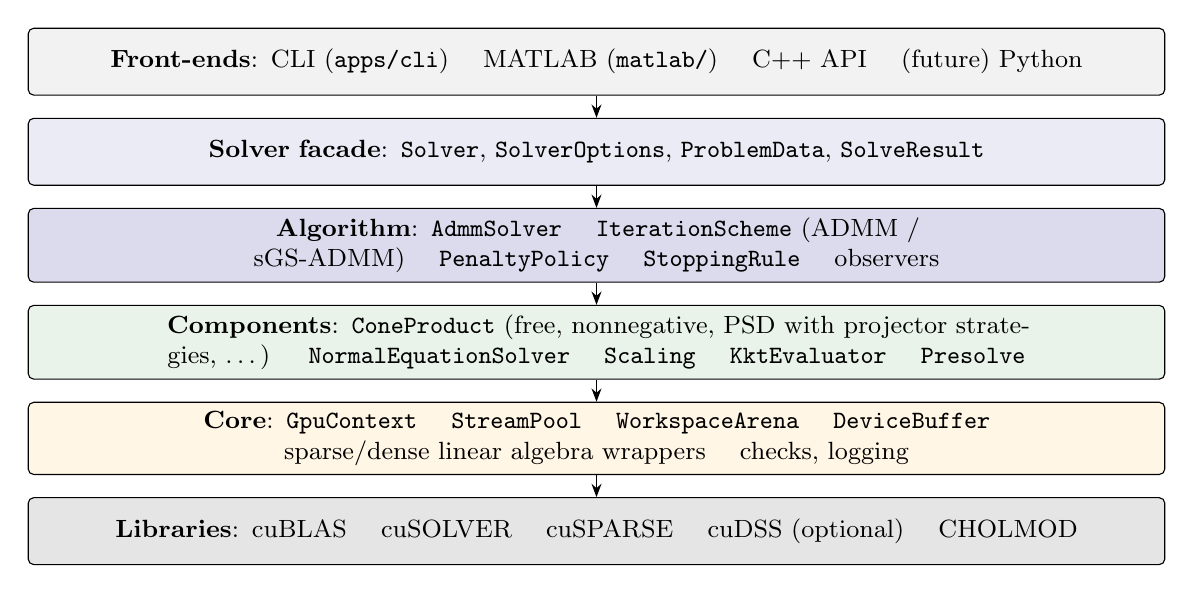
\begin{tikzpicture}[
  layer/.style={draw, rounded corners=2pt, minimum height=0.85cm, text width=14.2cm, align=center, font=\small},
  >=Stealth, node distance=0.28cm]
\node[layer, fill=Gray!10] (fe) {\textbf{Front-ends}: CLI (\texttt{apps/cli}) \quad MATLAB (\texttt{matlab/}) \quad C++ API \quad (future) Python};
\node[layer, fill=NavyBlue!8, below=of fe] (fa) {\textbf{Solver facade}: \texttt{Solver}, \texttt{SolverOptions}, \texttt{ProblemData}, \texttt{SolveResult}};
\node[layer, fill=NavyBlue!14, below=of fa] (al) {\textbf{Algorithm}: \texttt{AdmmSolver} \quad \texttt{IterationScheme} (ADMM / sGS-ADMM) \quad \texttt{PenaltyPolicy} \quad \texttt{StoppingRule} \quad observers};
\node[layer, fill=ForestGreen!10, below=of al] (co) {\textbf{Components}: \texttt{ConeProduct} (free, nonnegative, PSD with projector strategies, \dots) \quad \texttt{NormalEquationSolver} \quad \texttt{Scaling} \quad \texttt{KktEvaluator} \quad \texttt{Presolve}};
\node[layer, fill=Orange!10, below=of co] (core) {\textbf{Core}: \texttt{GpuContext} \quad \texttt{StreamPool} \quad \texttt{WorkspaceArena} \quad \texttt{DeviceBuffer} \quad sparse/dense linear algebra wrappers \quad checks, logging};
\node[layer, fill=Gray!20, below=of core] (lib) {\textbf{Libraries}: cuBLAS \quad cuSOLVER \quad cuSPARSE \quad cuDSS (optional) \quad CHOLMOD};
\foreach \a/\b in {fe/fa, fa/al, al/co, co/core, core/lib} \draw[->] (\a) -- (\b);
\end{tikzpicture}
\caption{Layers and dependency direction.}
\label{fig:layers}
\end{figure}

\subsection{Directory layout}
\begin{lstlisting}[style=plain]
cuADMM/
|-- CMakeLists.txt        CUADMM_WITH_{CUDSS,CHOLMOD}, CUADMM_BUILD_{CLI,MATLAB,TESTS,BENCH}
|-- cmake/                FindCUDSS.cmake, FindCHOLMOD.cmake, compiler warnings
|-- include/cuadmm/       public API only
|   |-- cuadmm.h          umbrella header
|   |-- options.h         SolverOptions (single source of defaults)
|   |-- problem.h         ProblemData, ConeSpec
|   |-- result.h          SolveResult, Status, Statistics
|   `-- solver.h          Solver facade
|-- src/
|   |-- core/             GpuContext, StreamPool, WorkspaceArena, buffers, checks, logging
|   |-- linalg/           sparse matrix wrappers (CSR/CSC), SpMV, vector kernels
|   |-- problem/          BlockLayout, Presolve (dependent rows, grouping by cone), DeviceProblem
|   |-- scaling/          Scaling
|   |-- cone/
|   |   |-- cone.h, cone_product.{h,cu}, cone_registry.{h,cu}
|   |   |-- free_cone.cu, nonnegative_cone.cu        (soc/ added in Phase 9)
|   |   `-- psd/
|   |       |-- psd_cone.{h,cu}, psd_block_group.h, svec.cu
|   |       |-- projectors/   one file per PSD projection strategy (catalog in Section 9)
|   |       |-- policy/       PsdProjectionPolicy, LargeBlockState, RankAnalyzer
|   |       `-- kernels/      composite filters + coefficients, Lanczos bound, LOBPCG
|   |-- linsys/           NormalMatrix, NormalEquationSolver, cudss/ cholmod/ dense/, factory
|   |-- admm/             AdmmState, IterationScheme, PenaltyPolicy, AdmmSolver
|   |-- termination/      KktEvaluator, StoppingRule, BestIterate, ExternalValidator, Certificate
|   |-- io/               TXT problem reader, solution and warm-start I/O
|   `-- report/           IterationObserver: console, CSV, sigma log, JSON, checkpoints
|-- apps/cli/             cuadmm executable (argument parser driven by the option table)
|-- matlab/               MEX gateway and +cuadmm package (options struct)
|-- test/                 unit/, integration/, golden/, data/
|-- bench/                projection and linear-system micro-benchmarks, end-to-end suites
|-- docs/                 this plan, design notes, Doxygen configuration
|-- examples/             unchanged
`-- experiments/          unchanged (frozen records of published runs)
\end{lstlisting}

\subsection{Naming and coding conventions}
\begin{center}\small
\begin{tabularx}{\textwidth}{@{}l>{\raggedright\arraybackslash}X@{}}
\toprule
Item & Convention \\
\midrule
Namespaces & \code{cuadmm}, \code{cuadmm::core}, \code{cuadmm::cone}, \code{cuadmm::cone::psd},
\code{cuadmm::linsys}, \code{cuadmm::admm}, \code{cuadmm::termination}, \code{cuadmm::report};
implementation details in \code{detail} or anonymous namespaces.\\
Files & \code{snake_case}, named after the main class (\code{full_evd_projector.cu} defines
\code{FullEvdProjector}); public headers only under \code{include/cuadmm}.\\
Types & \code{PascalCase} classes and structs; \code{enum class} with \code{PascalCase} values
(\code{IterationScheme::SgsAdmm}).\\
Functions, variables & \code{snake_case}; private members end in \code{_} (\code{sigma_}).\\
Constants & \code{constexpr} with a \code{k} prefix (\code{kDefaultTau}); no \texttt{\#define} for numerical
parameters---those are options.\\
CUDA kernels & \code{snake_case_kernel}, file-local (\code{static} or anonymous namespace), launched only
through a host wrapper that takes an \code{ExecContext}.\\
Math names & as in Appendix~\ref{app:notation}: \code{sigma}, \code{tau}, \code{y_step}, \code{cone_step},
\code{multiplier_step}, \code{eta_p}, \code{eta_d}, \code{eta_g}.\\
Errors & \code{CUADMM_CHECK_CUDA/CUBLAS/CUSOLVER/CUSPARSE/CUDSS} macros throwing \code{cuadmm::Error}
with call site and context; no \code{exit()} in library code.\\
Ownership & RAII for every CUDA object; non-owning \code{DeviceSpan<T>} for views; no raw
\code{cudaMalloc} outside \code{core}.\\
Style tools & \code{.clang-format}, \code{.clang-tidy}, Doxygen comments on every public type; warnings as
errors in CI.\\
\bottomrule
\end{tabularx}
\end{center}

\subsection{Public API}
\begin{lstlisting}
namespace cuadmm {

struct ConeSpec { ConeKind kind; std::int64_t size; double parameter = 0.0; };

struct ProblemData {                       // host data, original units
  CscMatrix At;                            // vec_len x m, transpose of A in svec form
  SparseVector b, C;
  std::vector<ConeSpec> cones;             // in input order
};

struct WarmStart { std::vector<double> X, y, S; std::optional<double> sigma; };

class Solver {
 public:
  explicit Solver(SolverOptions options);
  void setup(const ProblemData& problem);  // presolve, scale, factorize AA^T, plan cones
  SolveResult solve(const WarmStart* warm_start = nullptr);
  const SolverOptions& options() const;
  void add_observer(std::shared_ptr<report::IterationObserver> observer);
};

}  // namespace cuadmm
\end{lstlisting}
\code{SolveResult} carries the unscaled iterate, the residuals $\eta_p,\eta_d,\eta_g$, cone violations, the
certificate quantities, the stop reason, timings per phase and component, and the choices made at setup
(normal-equation backend, PSD strategies per block group).

%=======================================================================================================
\section{Algorithm layer}\label{sec:algorithm}

\subsection{The iteration loop}
After the reorganization the loop reads as the mathematics:
\begin{lstlisting}
SolveResult AdmmSolver::run(AdmmState& s) {
  for (int k = 1; ; ++k) {
    const KktResiduals r = kkt_.evaluate(s);               // original units, cached
    if (const auto stop = stopping_.check(k - 1, r, s)) return finish(*stop, s);
    scheme_->iterate(s, sigma_, tau_);                      // y-step(s), cone, multiplier
    sigma_ = penalty_->update(k, kkt_.evaluate(s), sigma_);
    observers_.on_iteration(k, s, r, sigma_);
  }
}
\end{lstlisting}

\subsection{Iteration schemes}
\begin{lstlisting}
class IterationScheme {
 public:
  virtual ~IterationScheme() = default;
  virtual std::string_view name() const = 0;
  // One iteration of (2)-(4) (ADMM) or its sGS variant.
  virtual void iterate(AdmmState& s, double sigma, double tau) = 0;
  virtual int normal_solves_per_iteration() const = 0;      // 1 for ADMM, 2 for sGS-ADMM
};
class AdmmScheme final : public IterationScheme { /* (2) -> (3) -> (4) */ };
class SgsAdmmScheme final : public IterationScheme { /* (2) -> (3) -> (2') -> (4) */ };
\end{lstlisting}
Both share the step implementations (\code{y_step}, \code{cone_step}, \code{multiplier_step}) in
\code{AdmmState}; the sGS scheme differs in one extra call. $\tau$ is validated in $(0,2)$ at setup.
An optional \code{scheme_switch_iteration} reproduces the hybrid mode.

\subsection{Penalty policies}
\begin{lstlisting}
class PenaltyPolicy {
 public:
  virtual ~PenaltyPolicy() = default;
  virtual std::string_view name() const = 0;
  virtual void reset(double sigma0) = 0;
  // Returns sigma for the next iteration; records every change for the sigma log.
  virtual double update(int k, const KktResiduals& r, double sigma) = 0;
};
class FixedPenalty final : public PenaltyPolicy { };             // sigma_k = sigma_0
class ResidualBalancingPenalty final : public PenaltyPolicy { };  // Section 3.5
class LegacyPenalty final : public PenaltyPolicy { };            // old rule, if Q1 keeps it
\end{lstlisting}
\code{ResidualBalancingPenalty} exposes the schedule, the factor (2), the ratio (1.35), the
$\max(1,\cdot)$ guard and the bounds as options and documents that $\sigma$ is in scaled units. The
\code{Monitor1} heuristic is deleted; if Q1 keeps a legacy policy, it lives only there.

\subsection{Termination and validation}
\begin{itemize}
  \item \code{KktEvaluator} computes $\eta_p,\eta_d,\eta_g$ once per iteration from the cached residual vectors
  and the \code{Scaling} object (no ad hoc unscaling).
  \item Stopping rules implement \code{StoppingRule}: the default \code{InternalKktRule}; the
  \code{ValidatedRule}, which is today's validation-aware stopping through the \code{ExternalValidator};
  and the \code{StrictDimacsRule}. All of them also enforce the iteration and time limits and detect
  non-finite residuals.
  \item \code{BestIterateTracker} keeps the best internal or externally validated iterate.
  \item \code{Certificate} computes the cone-measure terms of the certified lower bound through
  \code{Cone::measure} (Section~\ref{sec:cones}), so new cones contribute their own terms.
\end{itemize}

\subsection{Reporting}
All bookkeeping that today lives in solver fields (\code{info_*} arrays, \code{sigma_log}, phase timers,
validation history) moves to \code{IterationObserver} implementations: console table, CSV history,
$\sigma$ log, JSON summary, checkpoint writer. The solver emits events
(\code{on_setup}, \code{on_iteration}, \code{on_sigma_change}, \code{on_projection_switch},
\code{on_validation}, \code{on_finish}); observers never influence the iteration.

%=======================================================================================================
\section{Cones}\label{sec:cones}

\subsection{Interface}
\begin{lstlisting}
enum class ConeKind { Free, Nonnegative, Psd, SecondOrder, RotatedSecondOrder, Exponential, Power };

class Cone {
 public:
  virtual ~Cone() = default;
  virtual ConeKind kind() const = 0;
  virtual std::string_view name() const = 0;
  virtual std::int64_t dimension() const = 0;       // length of this cone's slice
  virtual bool is_self_dual() const = 0;
  virtual WorkspaceRequest workspace() const = 0;   // served by the WorkspaceArena
  // Cone step (3): s = Pi_{K*}(z) on this cone's slice.
  virtual void project_dual(DeviceSpan<const double> z, DeviceSpan<double> s, ExecContext& ctx) = 0;
  // Optional; default via Moreau: Pi_K(z) = z + Pi_{K*}(-z).
  virtual void project_primal(DeviceSpan<const double> z, DeviceSpan<double> x, ExecContext& ctx);
  // Violation measures and certificate coefficient of X (Side::Primal) or S (Side::Dual).
  virtual ConeMeasures measure(DeviceSpan<const double> v, Side side, ExecContext& ctx) = 0;
  virtual ScalingCompatibility scaling_compatibility() const = 0;
};
\end{lstlisting}
A \code{ConeProduct} owns one object per cone kind (each holding all blocks of that kind), maps slices of
the vector to cones, runs their \code{project_dual} on separate streams when profitable, and joins them
with events. A \code{ConeRegistry} maps input codes to factories, so the TXT reader, the MATLAB gateway
and the validator never switch on cone letters.

\subsection{Existing cones}
\begin{center}\small
\begin{tabularx}{\textwidth}{@{}lll>{\raggedright\arraybackslash}X@{}}
\toprule
Code & Primal $\K_\beta$ & Dual $\Kd_\beta$ & Cone step and status \\
\midrule
\code{s n} & $\Sym^n_+$ & $\Sym^n_+$ & $Q\max(\Lambda,0)Q^\top$ through the strategies of Section~\ref{sec:psd}; correct, tested for all tiers. \\
\code{l n} & $\R^n_+$ & $\R^n_+$ & $\max(z,0)$; correct, tested together with PSD and free blocks (a pure-LP test is added in Phase 5). \\
\code{u n} & $\R^n$ & $\{0\}$ & $s=0$; correct, tested alone and with PSD blocks. \\
\bottomrule
\end{tabularx}
\end{center}

\subsection{Adding a cone (checklist)}
\begin{enumerate}
  \item Implement a \code{Cone} subclass with \code{project_dual} (or \code{project_primal} plus Moreau) and \code{measure}.
  \item Register its input code and parameters in \code{ConeRegistry}.
  \item Add a generator case producing a problem with a known strictly complementary solution for the cone
  (the pattern of \code{test/regression_problems.hpp}).
  \item Add unit tests of the projection: idempotence, Moreau decomposition $z = \Proj_\K(z) - \Proj_{\Kd}(-z)$,
  orthogonality $\inner{\Proj_\K(z)}{\Proj_{\Kd}(-z)} = 0$, nonexpansiveness, and membership.
  \item Declare scaling compatibility and document the cone in the input-format section.
\end{enumerate}

\subsection{Planned cones}
\begin{itemize}
  \item \textbf{Second-order} $\mathcal{Q}^n = \{(t,x): \norm{x}\le t\}$ (code \code{q}), self-dual, closed form:
  $(t,x)$ if $\norm{x}\le t$; $0$ if $\norm{x}\le -t$; otherwise
  $\tfrac{t+\norm{x}}{2}\,(1, x/\norm{x})$. One batched kernel with a segmented reduction.
  \item \textbf{Rotated second-order} (code \code{r}) through the orthogonal map to $\mathcal{Q}^n$.
  \item \textbf{Exponential and power cones}: not self-dual, projections by a few Newton steps per cone;
  the interface already separates primal and dual projections.
\end{itemize}
The current scaling (row normalization of $\A$ and two scalars) is valid for every cone. Any future
variable scaling must be uniform on each PSD and second-order block; \code{scaling_compatibility()} makes
this checkable.

%=======================================================================================================
\section{PSD cone projection strategies}\label{sec:psd}

\subsection{Organization}
\code{PsdCone} groups its blocks into \code{PsdBlockGroup}s of equal size $n$ (stored as a contiguous batch of
$n\times n$ column-major matrices), converts the $\svec$ slice to the batch, projects, and converts back.
Each group has a \emph{size class} (small, medium, large) and is assigned a \code{PsdProjector}; large blocks
additionally carry a per-block \code{LargeBlockState} because their strategy changes during a run.
\begin{lstlisting}
struct PsdBatch { double* data; int n; int count; std::int64_t stride; };  // count n x n matrices

enum class ProjectionStatus { Ok, Rejected };  // Rejected: fall back to the exact projector

class PsdProjector {
 public:
  virtual ~PsdProjector() = default;
  virtual std::string_view name() const = 0;
  virtual WorkspaceRequest workspace(int n, int count) const = 0;
  // In place: M_i <- Pi_{S^n_+}(M_i) for every matrix of the batch.
  virtual ProjectionStatus project(PsdBatch batch, ExecContext& ctx) = 0;
};
\end{lstlisting}

\subsection{Strategy catalog}
Table~\ref{tab:psd-strategies} lists every projector. All of them exist in some form today; the
reorganization gives each one a name, a file, a workspace declaration and a test.

{\small
\begin{longtable}{@{}>{\raggedright\arraybackslash}p{3.5cm}>{\raggedright\arraybackslash}p{3.6cm}>{\raggedright\arraybackslash}p{1.4cm}>{\raggedright\arraybackslash}p{6.6cm}@{}}
\caption{PSD projection strategies (``Today'' refers to the baseline code).}\label{tab:psd-strategies}\\
\toprule
Projector & Method & Precision & Use, cost and notes\\
\midrule
\endfirsthead
\toprule
Projector & Method & Precision & Use, cost and notes\\
\midrule
\endhead
\code{JacobiBatchedEvdProjector} & \code{cusolverDnDsyevjBatched}, one call per size group & FP64 &
Small blocks ($n\le32$). Tolerance $10^{-16}$, 15 sweeps; \code{info = n+1} (tolerance not reached) is a
warning. Today: small tier.\\
\code{BatchedEvdProjector} & \code{cusolverDnXsyevBatched}, one call per size group & FP64 & Medium
groups ($32<n\le1000$) with at least two blocks, CUDA $\ge$ 12.8. Verified on the reference workstation up
to $n=1000$: residual $\approx4\times10^{-15}$, orthogonality $\approx10^{-13}$. Today: medium tier.\\
\code{StreamedEvdProjector} & \code{cusolverDnXsyevd} per block on $N$ streams & FP64 & Medium singletons, or
every medium block with CUDA $<$ 12.8. One workspace per block. Today: medium tier.\\
\code{FullEvdProjector} & \code{cusolverDnXsyevd}, then $Q\max(\Lambda,0)Q^\top$ & FP64 & Large blocks
($n>1000$) in the exact phase; also the fallback of every large strategy and the provider of eigenvalues
for \code{RankAnalyzer}. One stream; the final GEMM is batched per size group.\\
\code{LobpcgProjector} (\code{Positive}) & warm-started LOBPCG \cite{lobpcg} on $Z$, $P = V\max(D,0)V^\top$ & FP64 & Large
blocks whose positive rank is below $\rho n$; $k=\lceil 1.2\,r_+\rceil$ pairs. Cost $O(n^2k)$ per
LOBPCG iteration.\\
\code{LobpcgProjector} (\code{Negative}) & LOBPCG on $-Z$, $P = Z + V\max(D,0)V^\top$ & FP64 & Large blocks
whose negative rank is below $\rho n$ (primal low rank). Uses $\Proj(Z) = Z + \Proj(-Z)$.\\
\code{CompositeFilterProjector} (\code{Fp16}, \code{Fp32}, \code{Fp32Emulated}) & Lanczos bound, then the
composite polynomial filter of \cite{composite} & FP16 / FP32 / BF16x9 & Large blocks in the warm-up phase;
22 (FP16) or 31 (FP32) GEMMs. Rejected if not finite or if the norm test below fails.\\
\code{FullEvdFp32Projector} (optional) & \code{cusolverDnXsyevd} in FP32 & FP32 & Experimental; exists in the
submodule today, not wired into the solver.\\
\bottomrule
\end{longtable}
}

\subsection{Selection policy}
\code{PsdProjectionPolicy} assigns projectors from two inputs: the size class (thresholds are options:
\code{psd.small_max = 32}, \code{psd.medium_max = 1000}, \code{psd.medium_batch_min = 2}) and, for large
blocks, the phase of the run (Figure~\ref{fig:psd-state}). Unlike today, the warm-up switch and the start
of the low-rank analysis are two separate, explicit options; today both hang on
\code{switched_proj_method}, which is why the CLI default of 0 starts the rank analysis at iteration 2.

\begin{figure}[h]
\centering
\resizebox{\textwidth}{!}{%
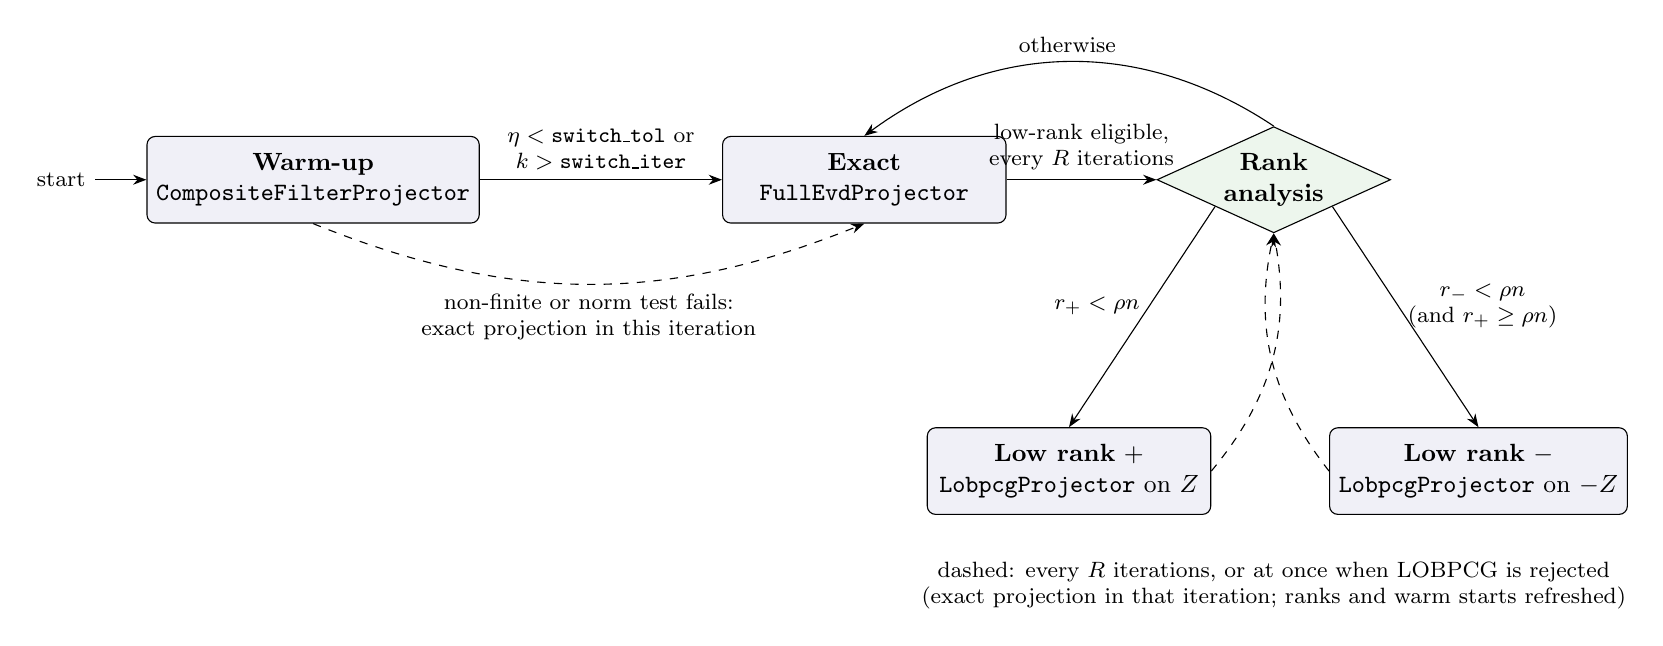
\begin{tikzpicture}[
  >=Stealth, font=\small,
  st/.style={draw, rounded corners=3pt, align=center, minimum width=3.6cm, minimum height=1.1cm, fill=NavyBlue!6},
  dc/.style={draw, diamond, aspect=2.2, align=center, inner sep=1pt, fill=ForestGreen!8},
  lab/.style={font=\footnotesize, align=center}]
\node[st] (W) at (0,0) {\textbf{Warm-up}\\ \texttt{CompositeFilterProjector}};
\node[st] (E) at (7.0,0) {\textbf{Exact}\\ \texttt{FullEvdProjector}};
\node[dc] (R) at (12.2,0) {\textbf{Rank}\\\textbf{analysis}};
\node[st] (Lp) at (9.6,-3.7) {\textbf{Low rank} $+$\\ \texttt{LobpcgProjector} on $Z$};
\node[st] (Ln) at (14.8,-3.7) {\textbf{Low rank} $-$\\ \texttt{LobpcgProjector} on $-Z$};
\node[lab] (S) at (-3.2,0) {start};
\draw[->] (S) -- (W);
\draw[->] (W) -- node[lab, above] {$\eta < \texttt{switch\_tol}$ or\\ $k > \texttt{switch\_iter}$} (E);
\draw[->, dashed] (W.south) to[bend right=22] node[lab, below] {non-finite or norm test fails:\\ exact projection in this iteration} (E.south);
\draw[->] (E) -- node[lab, above] {low-rank eligible,\\ every $R$ iterations} (R);
\draw[->] (R.north) to[bend right=35] node[lab, above] {otherwise} (E.north);
\draw[->] (R.south west) -- node[lab, left, pos=0.45] {$r_+ < \rho n$} (Lp.north);
\draw[->] (R.south east) -- node[lab, right, pos=0.45] {$r_- < \rho n$\\ (and $r_+ \ge \rho n$)} (Ln.north);
\draw[->, dashed] (Lp.east) to[bend right=25] (R.south);
\draw[->, dashed] (Ln.west) to[bend left=25] (R.south);
\node[lab] at (12.2,-5.15) {dashed: every $R$ iterations, or at once when LOBPCG is rejected\\
(exact projection in that iteration; ranks and warm starts refreshed)};
\end{tikzpicture}}
\caption{Per-block state machine for large PSD blocks. Without a warm-up method the block starts in
\textbf{Exact}. Rank analysis is a \texttt{FullEvdProjector} call plus \texttt{RankAnalyzer}; a rejected LOBPCG
result is replaced by an exact projection in the same iteration, which also refreshes ranks and warm starts.
Defaults: $\texttt{switch\_tol} = 10^{-2}$, $\rho = 0.03$, $R = 100$; \texttt{switch\_iter} is decision Q2.}
\label{fig:psd-state}
\end{figure}

\paragraph{Rank analysis.} With eigenvalues $\lambda_1\le\dots\le\lambda_n$ of the block,
\[
\text{tol}_r = \max\big(10^{-8}\max(|\lambda_1|,|\lambda_n|),\ 10^{-3}\,\text{tol}\big),\qquad
r_+ = \#\{\lambda_i>\text{tol}_r\},\qquad r_- = \#\{\lambda_i<-\text{tol}_r\}.
\]
Positive mode is preferred when both ranks are small. The top (or bottom) $k$ eigenpairs are kept as the
LOBPCG warm start.

\paragraph{LOBPCG acceptance.} A result is accepted if LOBPCG converged, all Ritz values are finite, and the
$k$-th Ritz value is at most $\text{tol}_r$ plus the residual norm. This is necessary, not sufficient (Ritz
values are lower bounds); the periodic exact analysis and the cone violation reported at termination bound
the risk. The tolerance becomes relative to the stopping tolerance (option, B13).

\subsection{Integrating the composite polynomial filter}\label{sec:composite}
\begin{enumerate}
  \item \textbf{Code move.} The composite kernels (FP16, FP32, FP32-emulated), the Lanczos norm bound
  (\code{approximate_two_norm}), LOBPCG and the precision-conversion and symmetrization helpers move to
  \code{src/cone/psd/kernels/}. The WIP functions (\code{compute_eigenpairs},
  \code{*_auto_scale_deflate}) and the commented-out coefficient candidates are not carried over; the
  standalone repository keeps them, and deflation is recorded as a possible future strategy.
  \item \textbf{Coefficients as data.} \code{constexpr} tables \code{kCompositeFp32[10][3]} and
  \code{kCompositeFp16[7][3]} hold the refined coefficients $\tilde f$ of \cite[Tables~1 and 2]{composite}
  (identical to the code today), obtained by Remez initialization and gradient refinement as in
  \cite{composite}, with the Polar Express coefficients \cite{polarexpress} kept only as a test baseline,
  and with a provenance comment. Each step evaluates
  $a X + b X^3 + c X^5$ with three GEMMs ($X^2$, $X^3$, $X^3X^2$).
  \item \textbf{Algorithm per block.} Lanczos (20 steps) on $Z^2$ gives $\theta$ and $q$;
  $u = \sqrt{\theta + \norm{Z^2q - \theta q}}$ \cite[Theorem~2]{composite}; scale $s = \mu u$ with safety
  margin $\mu = 1.02$ (FP32) or $1.05$ (FP16); $X_0 = Z/s$; $X_t = \tilde f_t(X_{t-1}/d_t)$ with damping
  $d_t = 1.001$ for $t\le8$ (FP32) and $d_t = 1.01$ for all $t$ (FP16); result
  $P = s\cdot\tfrac12 X_0(I + X_T)$, symmetrized. The damping location (input, as coded, versus output, as in
  \cite[\S3.4]{composite}) is documented and kept as coded (B11).
  \item \textbf{Precision and math modes (fixes B1).} One cuBLAS handle per precision mode, each with an
  explicit setting: FP32 uses \code{CUBLAS_DEFAULT_MATH}; FP16 uses \code{cublasGemmEx} with
  \code{CUBLAS_COMPUTE_32F_FAST_16F} (unchanged); FP32-emulated uses
  \code{CUBLAS_FP32_EMULATED_BF16X9_MATH} with an emulation strategy (to be validated on a Blackwell GPU;
  the reference workstation cannot run it). \code{CUBLAS_TENSOR_OP_MATH} is never set.
  \item \textbf{Safety checks.} Reject (and fall back to \code{FullEvdProjector}) if the result is not
  finite or if $\norm{P}_F > (1+10^{-2})\norm{Z}_F$, a free necessary condition since the projection is
  nonexpansive with $\Proj(0)=0$. This also catches finite but wrong results from an underestimated scale.
  \item \textbf{Determinism (fixes B8).} The Lanczos start vector is drawn from a counter-based generator
  seeded by \code{(options.seed, block index)}, so runs are reproducible.
  \item \textbf{Workspace (fixes B7).} $3n^2$ floats (plus $3n^2$ halves for FP16) for the largest large
  block, and the Lanczos vectors, come from the \code{WorkspaceArena}; nothing is allocated per call.
  \item \textbf{Exposure (fixes B4).} Option \code{psd.large.warmup} $\in$ \{\code{none},
  \code{composite_fp16}, \code{composite_fp32}, \code{composite_fp32_emulated}\}, available in the CLI
  (\code{--psd-warmup}) and MATLAB (\code{opts.psd.large.warmup}). The default is decision Q3.
  \item \textbf{Scope.} The filter is used for large blocks only: its GEMM advantage needs $n$ in the
  thousands \cite{composite}, while many small blocks are served better by batched EVD. A strided-batched
  composite filter for medium groups is a benchmark item, not a default.
\end{enumerate}

\subsection{LOBPCG improvements}
\begin{itemize}
  \item Preallocate per-block workspaces (B7); keep the eigenpair warm starts in the
  \code{LargeBlockState}.
  \item Reuse $Z X_k$ from the residual computation in the Rayleigh--Ritz step instead of recomputing it
  inside $Q^\top Z Q$.
  \item Negative mode: pass $\alpha=-1$ to the GEMMs instead of negating the block in place twice.
  \item Options for maximum iterations (20), tolerance (relative to $\text{tol}$), ratio $\rho$ (0.03),
  relaxation (1.2) and re-evaluation period $R$ (100), all reported in the summary.
\end{itemize}

\subsection{PSD options}
\begin{center}\small
\begin{tabularx}{\textwidth}{@{}l l>{\raggedright\arraybackslash}X@{}}
\toprule
Option & Default & Today\\
\midrule
\code{psd.small_max}, \code{psd.medium_max} & 32, 1000 & \code{SMALL_MAT_LIMIT}, \code{MEDIUM_MAT_LIMIT} macros\\
\code{psd.medium_batch_min} & 2 & public field \code{medium_batch_min_count}\\
\code{psd.medium_streams} & 15 & \code{--streams}, first MEX argument\\
\code{psd.jacobi_tol}, \code{psd.jacobi_max_sweeps} & $10^{-16}$, 15 & constructor defaults of \code{BatchEigParameter}\\
\code{psd.large.warmup} & Q3 & hard-coded \code{EIG_FP64}\\
\code{psd.large.switch_tol}, \code{psd.large.switch_iter} & $10^{-2}$, Q2 & $10^{-2}$; CLI 0 / MATLAB 5000\\
\code{psd.lowrank.enabled} & true & \code{--lobpcg}\\
\code{psd.lowrank.start_tol}, \code{psd.lowrank.start_iter} & $= $ switch values & coupled to the warm-up switch\\
\code{psd.lowrank.ratio}, \code{.relaxation}, \code{.reevaluate} & 0.03, 1.2, 100 & \code{LOBPCG_*} macros\\
\code{psd.lowrank.max_iter}, \code{.tol} & 20, relative & 20, absolute $10^{-5}$\\
\code{psd.lowrank.rank_rtol}, \code{.rank_stop_factor} & $10^{-8}$, $10^{-3}$ & macros\\
\code{psd.composite.margin_fp32}, \code{.margin_fp16} & 1.02, 1.05 & \code{COMPOSITE_*_SCALE_MARGIN} macros\\
\code{psd.composite.lanczos_steps}, \code{.seed} & 20, 0 & 20, random seed\\
\bottomrule
\end{tabularx}
\end{center}

%=======================================================================================================
\section{Normal-equation solvers}\label{sec:linsys}

\subsection{Role}
Every y-step solves $(\A\Ad + \varepsilon I)\,y = r$ with the scaled, row-normalized $\A$; ADMM needs one solve
per iteration and sGS-ADMM two. The matrix does not depend on $\sigma$, so analysis and factorization run
once at setup and the \emph{solve} time dominates. Today CHOLMOD \cite{cholmod} always factors on the CPU (supernodal,
falling back to simplicial $LDL^\top$); solves run on the CPU with a device synchronization and two
PCIe copies per iteration, unless the factor is dense ($m\ge2000$,
$\mathrm{nnz}(L) > 0.3\,m(m+1)/2$, $8m^2$ bytes $\le$ 25\% of free memory), in which case $L$ and $D$ are
copied to the GPU and each solve is two \code{cublasDtrsv} calls.

\subsection{Interface}
\begin{lstlisting}
class NormalEquationSolver {
 public:
  virtual ~NormalEquationSolver() = default;
  virtual std::string_view name() const = 0;
  virtual SymbolicInfo analyze(const NormalMatrix& AAt) = 0;   // ordering, nnz(L), memory
  virtual FactorInfo factorize(const NormalMatrix& AAt) = 0;   // numeric, pivot statistics
  virtual void solve(DeviceSpan<const double> rhs, DeviceSpan<double> y, ExecContext& ctx) = 0;
  virtual bool solves_on_device() const = 0;
};
\end{lstlisting}
\code{NormalMatrix} builds $\A\Ad+\varepsilon I$ once (lower triangle, CSR), on the GPU with
\code{cusparseSpGEMM} or on the host with \code{cholmod_aat}, and records pivot statistics for diagnostics.

\subsection{Backends}
\begin{description}
  \item[\code{CudssSolver} (preferred).] NVIDIA cuDSS \cite{cudss}, distributed separately from the CUDA toolkit; it is
  NVIDIA's replacement for the sparse Cholesky routines of cuSOLVER, which the CUDA 12.9 headers mark
  deprecated in favor of cuDSS (\code{cusolverSpDcsrlsvchol}, \code{cusolverSpXcsrchol*}). Phases:
  analysis (reordering, symbolic), factorization, solve, all on the device; matrix type SPD (Cholesky) or
  symmetric indefinite ($LDL^\top$) for rank-deficient data; lower view; solves on the solver stream with no
  host synchronization. Enabled by \code{CUADMM_WITH_CUDSS}; the exact API calls and the minimum version
  are pinned when the backend is written.
  \item[\code{CholmodSolver} (always available).] Today's behavior, moved out of \code{SDPSolver}:
  supernodal with simplicial $LDL^\top$ fallback; CPU solves through pinned host buffers and asynchronous
  copies on the solver stream; the dense-GPU-triangular-solve mode is kept as an option of this backend.
  \item[\code{DenseCusolverSolver} (optional).] \code{cusolverDnXpotrf}/\code{cusolverDnXpotrs} for SPD,
  \code{cusolverDnDsytrf}/\code{cusolverDnXsytrs} otherwise; or an explicit inverse factor from
  \code{cusolverDnXtrtri} so each solve is two triangular matrix--vector products, which parallelize better
  than \code{trsv}. Useful when $m$ is a few thousand and the factor is dense.
  \item[\code{PcgSolver} (future).] Matrix-free conjugate gradients on $\A\Ad$ with warm start from the
  previous $y$, for problems whose factor does not fit; inexact solves are compatible with ADMM when the
  errors are summable.
\end{description}

\subsection{Selection}
\begin{enumerate}
  \item If \code{linsys.backend} is not \code{auto}, use it.
  \item Otherwise run the symbolic analysis (cuDSS analysis phase, or \code{cholmod_analyze}) to get
  $\mathrm{nnz}(L)$ and the memory need.
  \item If cuDSS is built in and its factor fits in the memory budget, use \code{CudssSolver}.
  \item Otherwise use \code{CholmodSolver}, with GPU dense solves if $8m^2$ bytes fit the budget and
  $\mathrm{nnz}(L)\ge0.3\,m(m+1)/2$, and CPU solves otherwise.
  \item With \code{linsys.autotune = true}, factor with the two best candidates, time ten solves each and keep
  the faster. The choice and the timings go to the log and the summary.
\end{enumerate}

\subsection{Rank deficiency and presolve}
Moment relaxations often have dependent constraints (the SPOT data); a tiny regularization
$\varepsilon = 10^{-15}$ plus simplicial $LDL^\top$ is what makes them work today, and it is fragile (B9).
A \code{Presolve} step detects dependent rows from the factorization pivots (or a sparse QR), removes them
after checking that $b$ is consistent, and maps $y$ back at the end. Regularization stays as a fallback
option (\code{linsys.regularization}). cuDSS in SPD mode also requires a nonsingular matrix, so presolve or
the $LDL^\top$ mode is needed there too.

\subsection{Benchmark protocol}
Problems: SPOT (PushBox, PushT, PlanarHand at $N=1,10,30$), pendulum (\code{licols}), and PLATO / Mittelmann
instances including one with a dense factor (\code{neosfrbr25}). Metrics: analysis, factorization and
per-solve time; peak memory; relative residual $\norm{\A\Ad y - r}/\norm{r}$; end-to-end time to
$\eta<10^{-4}$. GPUs: the RTX 6000 Ada workstation (FP64 throughput is about 1/64 of FP32, which penalizes
dense FP64 factorizations and FP64 EVD) and an H100/H200 node. Defaults are set from these results.

%=======================================================================================================
\section{Scaling}\label{sec:scaling}
A \code{Scaling} object holds $\nu$, $b_s$, $C_s$ and provides \code{scale_problem}, \code{scale_iterate},
\code{unscale_iterate}, \code{to_original_residuals} and \code{sigma_to_original}. It is the only code that
knows the scaling; the warm start, the termination, the validator and the result use it. Option
\code{scaling.enabled} (default true) allows running unscaled for diagnostics. The unused fields
\code{bscale2}, \code{Cscale2} are deleted.

%=======================================================================================================
\section{Core infrastructure}\label{sec:core}
\begin{itemize}
  \item \textbf{\code{GpuContext}}: device, library handles per stream role, cuDSS handle, and the
  math-mode policy of each handle set explicitly at creation.
  \item \textbf{\code{StreamPool} and \code{ExecContext}}: named streams (main, small, medium[$N$], large,
  linsys, copy). An \code{ExecContext} bundles a stream, its handles and a workspace slice; cross-stream
  dependencies use events. Everything runs on non-blocking streams owned by the pool, which removes the
  class of bugs behind B2.
  \item \textbf{\code{WorkspaceArena}}: components declare \code{WorkspaceRequest}s at setup; the arena
  allocates once and hands out aligned slices. No \code{cudaMalloc}/\code{cudaFree} inside the loop.
  \item \textbf{Buffers}: \code{DeviceBuffer<T>}, \code{PinnedHostBuffer<T>}, \code{DeviceSpan<T>} with
  \code{std::size_t} sizes; the overflow checks of \code{BlockStructure} are kept.
  \item \textbf{Determinism}: option \code{determinism} $\in$ \{\code{strict} (default), \code{fast}\}.
  \item \textbf{Logging}: a \code{Logger} with levels; library code does not call \code{printf}.
\end{itemize}

%=======================================================================================================
\section{Unified options}\label{sec:options}
Table~\ref{tab:options} is the single table of defaults (PSD options are in Section~\ref{sec:psd}). The CLI
flag names are derived from it (\code{algorithm.tau} becomes \code{--tau}, with the current flags kept as
aliases for one release) and the MATLAB options struct uses the same nested field names.

{\small
\begin{longtable}{@{}>{\raggedright\arraybackslash}p{6.3cm}>{\raggedright\arraybackslash}p{3.5cm}>{\raggedright\arraybackslash}p{5.9cm}@{}}
\caption{Solver options and defaults (``Q'' marks an open decision of Section~\ref{sec:decisions}).}\label{tab:options}\\
\toprule
Option & Default & Notes\\
\midrule
\endfirsthead
\toprule
Option & Default & Notes\\
\midrule
\endhead
\code{algorithm.scheme} & \code{admm} & \code{admm} or \code{sgs_admm}; replaces \code{switch_admm} and the compile flag.\\
\code{algorithm.tau} & 1.618 & Validated in $(0,2)$; preset \code{--aggressive} sets 1.918 (Q4).\\
\code{algorithm.scheme_switch_iteration} & 0 (off) & Hybrid mode: sGS until this iteration, then ADMM.\\
\code{algorithm.max_iter}, \code{.time_limit} & $10^6$, none & As today in the CLI.\\
\code{algorithm.tol} & $10^{-4}$ & Internal stopping tolerance on $\eta$.\\
\code{penalty.policy} & \code{residual_balancing} & \code{fixed}, \code{residual_balancing}, \code{legacy} (Q1).\\
\code{penalty.sigma0} & 100 & Scaled units (Section~\ref{sec:math-scaling}).\\
\code{penalty.sigma_min}, \code{.sigma_max} & $10^{-3}$, $10^{3}$ & October 13 values.\\
\code{penalty.factor}, \code{.ratio}, \code{.guard} & 2, 1.35, true & The $\max(1,\cdot)$ guard is \code{guard}.\\
\code{penalty.schedule} & as in \S\ref{sec:penalty} & List of (up to iteration, period) pairs.\\
\code{scaling.enabled} & true & \\
\code{linsys.backend} & \code{auto} & \code{auto}, \code{cudss}, \code{cholmod}, \code{dense}.\\
\code{linsys.regularization} & $10^{-15}$ & Added to the diagonal of $\A\Ad$.\\
\code{linsys.presolve} & true & Remove dependent rows.\\
\code{linsys.memory_fraction}, \code{.autotune} & 0.25, false & Budget for dense or cuDSS factors.\\
\code{validation.interval}, \code{.tol}, \code{.threads} & 0, \code{tol}, 1 & Validation-aware stopping as today.\\
\code{output.verbosity}, \code{.history}, \code{.summary}, \code{.sigma_log} & 1, off, off, off & Observers.\\
\code{seed}, \code{determinism} & 0, \code{strict} & \\
\bottomrule
\end{longtable}
}

%=======================================================================================================
\section{Testing, benchmarking and continuous integration}\label{sec:testing}
\begin{itemize}
  \item \textbf{Unit tests} per component: cone properties (idempotence, Moreau decomposition, orthogonality,
  nonexpansiveness, membership); every PSD projector against an FP64 reference on synthetic spectra
  (full rank, low rank $\pm$, clustered, tiny $n$, $n=1000$ and $n>1000$), with tolerances per precision
  (FP32 composite below $10^{-4}$ median relative error, FP16 composite below $2\times10^{-3}$; exact
  projectors near machine precision); normal-equation solvers on full-rank and rank-deficient matrices;
  penalty policies on scripted residual sequences; option parsing and validation.
  \item \textbf{Integration tests}: generated problems with known optimum for every cone and every
  projector path, both schemes, $\tau\in\{1.618, 1.918\}$, both normal-equation backends.
  \item \textbf{Golden histories}: per-iteration $(\text{pobj},\text{dobj},\eta_p,\eta_d,\sigma)$ of a fixed set
  of problems, regenerated only by a documented script when a behavior change is intended (B14).
  \item \textbf{End-to-end}: a small SPOT and PLATO subset checked against MOSEK objective values.
  \item \textbf{Benchmarks} (\code{bench/}): projector micro-benchmarks, normal-equation backends,
  end-to-end time; results stored per GPU and compared release to release.
  \item \textbf{CI}: build matrix with and without cuDSS and CHOLMOD; CUDA 12.8 and 12.9; nightly
  \code{compute-sanitizer} (memcheck, racecheck, synccheck) on the integration tests; GPU runners for Ada
  and Hopper where available.
\end{itemize}

%=======================================================================================================
\section{Migration plan}\label{sec:migration}
Each phase is one or a few pull requests on a feature branch, reviewed and merged in order. ``Bitwise''
means identical per-iteration histories on the golden set and on two real problems.

\begin{description}[style=nextline,leftmargin=0.6cm]
\item[Phase 0 --- Safety net.] Freeze baseline histories (golden set plus one SPOT and one PLATO problem)
from \code{main} with the penalty rule chosen in Q1; add the CI build matrix; make the CHOLMOD
rank-deficient test independent of the SuiteSparse version (B9: skip with a message, or presolve later).
\emph{Acceptance:} CI green; baseline artifacts stored.
\item[Phase 1 --- Cleanup.] Delete dead code (P4); remove \code{CUADMM_PLAIN_ADMM_ONLY} (sGS back as a runtime
option, B5); fix B1 (math mode), B2 (event before the copy), B6, B12; update the README.
\emph{Acceptance:} bitwise on the exact paths; composite accuracy test tightened to FP32 levels.
\item[Phase 2 --- Options and front-ends.] \code{SolverOptions}, the \code{Solver} facade over the existing
class, CLI and MATLAB rebuilt on it; resolve B3 and B4 with the Q2/Q3 defaults; old flags as aliases.
\emph{Acceptance:} bitwise for equivalent options; option table generated into the documentation.
\item[Phase 3 --- Core infrastructure.] \code{GpuContext}, \code{StreamPool}, \code{ExecContext},
\code{WorkspaceArena}, buffers; LOBPCG and Lanczos stop allocating per call (B7).
\emph{Acceptance:} bitwise; no \code{cudaMalloc} in the loop (checked with Nsight Systems); sanitizers clean.
\item[Phase 4 --- Algorithm layer.] \code{AdmmState}, \code{IterationScheme} (ADMM, sGS-ADMM),
\code{PenaltyPolicy}, \code{KktEvaluator}, \code{StoppingRule}, \code{BestIterateTracker}, observers;
\code{solve()} becomes \code{AdmmSolver::run}. \emph{Acceptance:} bitwise for ADMM; sGS-ADMM matches the
pre-flag code; $\tau$ validation tests.
\item[Phase 5 --- Cone layer.] \code{Cone}, \code{ConeProduct}, \code{ConeRegistry}; free and nonnegative
cones; the PSD cone wrapping the current tiers unchanged; validator and certificate through
\code{Cone::measure}; pure-LP test. \emph{Acceptance:} bitwise.
\item[Phase 6 --- PSD strategies and composite integration.] The projector classes of
Table~\ref{tab:psd-strategies}, \code{PsdProjectionPolicy}, \code{LargeBlockState}, \code{RankAnalyzer};
submodule code moved in, B8, B10, B11, B13 addressed; submodule removed from \code{.gitmodules}.
\emph{Acceptance:} bitwise on exact and LOBPCG paths; composite accuracy and fallback tests; end-to-end
runs with each warm-up method reach the tolerance.
\item[Phase 7 --- Normal-equation solvers.] \code{NormalMatrix}, \code{NormalEquationSolver},
\code{CholmodSolver} (bitwise with today), \code{CudssSolver}, optional \code{DenseCusolverSolver},
selection and presolve; benchmark report. \emph{Acceptance:} CHOLMOD path bitwise; cuDSS path within
$10^{-10}$ relative residual per solve and same iteration counts within a few percent end to end.
\item[Phase 8 --- Data layout.] Permute variables at setup so each cone, and each PSD size group, owns a
contiguous slice; run cone projections concurrently on their streams. \emph{Acceptance:} within rounding
(summation order changes); speedup measured.
\item[Phase 9 --- New cones.] Second-order and rotated second-order cones with generator-based tests;
input format and MATLAB \code{K.q}/\code{K.r} fields. \emph{Acceptance:} new tests, CBLIB/DIMACS
second-order instances solved to tolerance.
\item[Phase 10 --- Documentation and release.] README rewrite, Doxygen, examples updated to the new options,
migration notes for users of the old MEX signature, tagged release.
\end{description}

\begin{warnbox}{Risks and mitigations}
\begin{itemize}[leftmargin=*]
  \item \emph{Silent behavior changes during refactoring} --- bitwise acceptance on the golden set for
  Phases 1--6; any intended change gets its own pull request and regenerated goldens.
  \item \emph{cuDSS availability and version drift} --- optional dependency behind
  \code{CUADMM_WITH_CUDSS}; CHOLMOD remains the guaranteed backend; the version is pinned in CMake.
  \item \emph{Performance regressions from abstraction} --- virtual calls happen once per component per
  iteration, not per element; benchmarks run in CI on every phase.
  \item \emph{Reproducing published results} --- \code{experiments/} records keep the commit hashes they used;
  a \code{legacy} penalty policy is kept if Q1 requires it.
\end{itemize}
\end{warnbox}

%=======================================================================================================
\section{Open decisions}\label{sec:decisions}
\begin{enumerate}[label=\textbf{Q\arabic*.}]
  \item \textbf{Penalty rule history.} Regenerate the golden histories with the October 13 rule, and keep a
  \code{legacy} policy (old rule, $[10^{-6},10^{6}]$, monitor) only if earlier results must be reproduced
  from the new code?
  \item \textbf{Warm-up switch iteration.} Default \code{switch_iter} of 5000 (MATLAB today) or 0 (CLI today),
  and should the start of the low-rank analysis be decoupled from it as proposed?
  \item \textbf{Default warm-up for large blocks.} \code{none} (today's effective behavior) or
  \code{composite_fp16}, as in the warm-start experiments of \cite{composite}?
  \item \textbf{Default $\tau$.} Keep 1.618 or make 1.918 the default after benchmarking.
  \item \textbf{Hybrid mode.} Keep \code{scheme_switch_iteration} (cheap given \cite{afterimage}) or drop it.
  \item \textbf{MATLAB interface.} Keep the positional MEX signature as a compatibility wrapper, or move to
  \code{cuadmm.solve(At, b, C, K, opts)} only.
  \item \textbf{cuDSS distribution.} Minimum version, and whether to use the system, conda or pip package.
  \item \textbf{Python bindings.} In scope for this reorganization or later?
  \item \textbf{Standalone \code{psd_projection} repository.} Keep it for the benchmarks of \cite{composite}
  (frozen), with cuADMM as the maintained home of the kernels?
\end{enumerate}

%=======================================================================================================
\appendix
\section{Mapping from current files to the new layout}\label{app:mapping}
{\small
\begin{longtable}{@{}>{\raggedright\arraybackslash}p{6.0cm}>{\raggedright\arraybackslash}p{6.0cm}>{\raggedright\arraybackslash}p{3.2cm}@{}}
\toprule
Current & New & Note\\
\midrule
\endfirsthead
\toprule
Current & New & Note\\
\midrule
\endhead
\code{SDPSolver} (\code{solver.h}, \code{solver.cu}) & \code{Solver} facade + \code{admm/}, \code{cone/}, \code{linsys/}, \code{termination/}, \code{report/} & split\\
\code{SDPSolver::init} & \code{Solver::setup}: \code{problem/}, \code{scaling/}, \code{linsys/} factory, \code{ConeProduct} planning & \\
\code{SDPSolver::solve} (loop) & \code{admm/AdmmSolver::run} & \\
y-step code, \code{solve_AAt_perm} & \code{AdmmState::y_step}, \code{linsys/cholmod/} & \\
\code{large_full_eig_project} & \code{FullEvdProjector} + \code{RankAnalyzer} & \\
\code{large_lobpcg_project} & \code{LobpcgProjector} & \\
\code{large_composite_project} & \code{CompositeFilterProjector} & \\
medium and small tiers (inline) & \code{BatchedEvdProjector}, \code{StreamedEvdProjector}, \code{JacobiBatchedEvdProjector} & \\
\code{cone_measures}, \code{certified_lower_bound} & \code{Cone::measure}, \code{termination/Certificate} & \\
\code{validate_current_iterate}, \code{external_validation.*} & \code{termination/ExternalValidator}, \code{ValidatedRule} & \\
$\sigma$ update in \code{solve}, \code{monitors.h} & \code{admm/PenaltyPolicy} & monitor deleted\\
best-iterate fields & \code{BestIterateTracker} & \\
\code{info_*} arrays, \code{sigma_log}, phase timers & \code{report/} observers & \\
\code{memory.h} & \code{core/device_buffer.h}, \code{core/handles.h}, \code{linalg/sparse_matrix.h} & \\
\code{check.h} & \code{core/check.h} & \\
\code{cublas.h}, \code{cusparse.h}, \code{cusolver.h} & \code{linalg/} wrappers, projector files & \\
\code{kernels/*.cu} & \code{linalg/vector_ops.cu}, \code{cone/psd/svec.cu}, \code{linsys/permutation.cu} & \\
\code{kernels/type_conversion.cu} & \code{matlab/} & MEX index conversion\\
\code{block_structure.*}, \code{matrix_sizes.*} & \code{problem/BlockLayout}, \code{cone/psd/PsdBlockGroup} & \\
\code{utils/analyze_blk.cu}, \code{utils/get_maps.cu}, \code{MatrixSizes::init}, \code{utils/get_eig_rank_mask.cu}, \code{utils/check_gpus.cu}, \code{max_dense_vector_zero_mask} & --- & deleted (unused)\\
\code{rank.cu} & \code{cone/psd/policy/RankAnalyzer} & \\
\code{cholesky_cpu.h} & \code{linsys/cholmod/CholmodSolver} & \\
\code{eig_cpu.h} & \code{test/} helper & test-only\\
\code{io.*}, \code{problem.*} & \code{io/}, \code{problem/} & \\
\code{main.cu} & \code{apps/cli/} & \\
\code{MATLAB/cuadmm_MATLAB.cu} & \code{matlab/} & \\
\code{psd_projection/src/composite_FP16.cu}, \code{composite_FP32.cu}, \code{composite_FP32_emulated.cu} & \code{cone/psd/kernels/composite_*.cu} & \\
\code{psd_projection/src/lanczos.cu} & \code{cone/psd/kernels/lanczos_bound.cu} & only the norm bound\\
\code{psd_projection/src/lobpcg.cu} & \code{cone/psd/kernels/lobpcg.cu} & \\
\code{psd_projection/src/utils.cu} & \code{cone/psd/kernels/precision.cu}, \code{symmetrize.cu} & \\
\code{psd_projection/src/eig_FP64_psd.cu}, \code{eig_FP32_psd.cu} & \code{FullEvdFp32Projector} (optional) & \\
\code{psd_projection/test/*} & \code{test/unit/psd/} & \\
\bottomrule
\end{longtable}
}

\section{Notation and code names}\label{app:notation}
\begin{center}\small
\begin{tabular}{@{}lll@{}}
\toprule
Symbol & Meaning & Code name\\
\midrule
$X$, $y$, $S$ & primal variable, dual multiplier, dual slack & \code{X}, \code{y}, \code{S}\\
$\A$, $\Ad$ & constraint map and adjoint & \code{A}, \code{At}\\
$\A\Ad$ & normal matrix & \code{NormalMatrix}\\
$\K$, $\Kd$ & cone and dual cone & \code{Cone}, \code{project_dual}\\
$\sigma$, $\tau$ & penalty, step length & \code{sigma}, \code{tau}\\
\eqref{eq:ystep}, \eqref{eq:sstep}, \eqref{eq:xstep} & the three steps & \code{y_step}, \code{cone_step}, \code{multiplier_step}\\
$\eta_p,\eta_d,\eta_g,\eta$ & residuals & \code{eta_p}, \code{eta_d}, \code{eta_g}, \code{eta}\\
$\nu$, $b_s$, $C_s$ & scaling factors & \code{Scaling::row_norms}, \code{b_scale}, \code{c_scale}\\
$r_+$, $r_-$, $\text{tol}_r$ & ranks and rank tolerance & \code{RankAnalyzer}\\
$\rho$, $R$ & low-rank ratio, re-evaluation period & \code{psd.lowrank.ratio}, \code{.reevaluate}\\
\bottomrule
\end{tabular}
\end{center}

%=======================================================================================================
\begin{thebibliography}{99}

\bibitem{cuadmm}
A.~Groudiev, S.~Kang, and H.~Yang.
\newblock cuADMM: GPU-accelerated first-order optimization for large-scale multi-block semidefinite programs.
\newblock In \emph{RSS Workshop on Fast Motion Planning and Control in the Era of Parallelism}, 2025.
\newblock \url{https://agroudiev.github.io/assets/pdf/8_cuADMM_GPU_Accelerated_First.pdf}.

\bibitem{composite}
S.~Kang, H.~Han, A.~Groudiev, and H.~Yang.
\newblock Factorization-free orthogonal projection onto the positive semidefinite cone with composite
polynomial filtering.
\newblock arXiv:2507.09165, 2025 (v2, 2026).

\bibitem{afterimage}
S.~Kang and H.~Yang.
\newblock Afterimage slow regions in first-order methods for linear conic programming.
\newblock arXiv:2609.09449, 2026.

\bibitem{wafr}
S.~Kang, X.~Xu, J.~Sarva, L.~Liang, and H.~Yang.
\newblock Fast and certifiable trajectory optimization.
\newblock In \emph{International Workshop on the Algorithmic Foundations of Robotics (WAFR)}, 2024.
\newblock arXiv:2406.05846.

\bibitem{kang2025local}
S.~Kang, X.~Jiang, and H.~Yang.
\newblock Local linear convergence of the alternating direction method of multipliers for semidefinite
programming under strict complementarity.
\newblock arXiv:2503.20142, 2025.

\bibitem{chen2017}
L.~Chen, D.~Sun, and K.-C. Toh.
\newblock An efficient inexact symmetric Gauss--Seidel based majorized ADMM for high-dimensional convex
composite conic programming.
\newblock \emph{Mathematical Programming}, 161(1--2):237--270, 2017.

\bibitem{chen2021}
L.~Chen, X.~Li, D.~Sun, and K.-C. Toh.
\newblock On the equivalence of inexact proximal ALM and ADMM for a class of convex composite programming.
\newblock \emph{Mathematical Programming}, 185(1):111--161, 2021.

\bibitem{gabay}
D.~Gabay and B.~Mercier.
\newblock A dual algorithm for the solution of nonlinear variational problems via finite element
approximation.
\newblock \emph{Computers \& Mathematics with Applications}, 2(1):17--40, 1976.

\bibitem{wen}
Z.~Wen, D.~Goldfarb, and W.~Yin.
\newblock Alternating direction augmented Lagrangian methods for semidefinite programming.
\newblock \emph{Mathematical Programming Computation}, 2(3):203--230, 2010.

\bibitem{sdpnalplus}
D.~Sun, K.-C. Toh, Y.~Yuan, and X.-Y. Zhao.
\newblock SDPNAL+: A Matlab software for semidefinite programming with bound constraints (version 1.0).
\newblock \emph{Optimization Methods and Software}, 35(1):87--115, 2020.

\bibitem{cholmod}
Y.~Chen, T.~A. Davis, W.~W. Hager, and S.~Rajamanickam.
\newblock Algorithm 887: CHOLMOD, supernodal sparse Cholesky factorization and update/downdate.
\newblock \emph{ACM Transactions on Mathematical Software}, 35(3), 2008.

\bibitem{cudss}
NVIDIA Corporation.
\newblock cuDSS: NVIDIA CUDA direct sparse solver library, documentation.
\newblock \url{https://docs.nvidia.com/cuda/cudss/}.

\bibitem{polarexpress}
N.~Amsel, D.~Persson, C.~Musco, and R.~Gower.
\newblock The Polar Express: optimal matrix sign methods and their application to the Muon algorithm.
\newblock arXiv:2505.16932, 2025.

\bibitem{lobpcg}
A.~V. Knyazev.
\newblock Toward the optimal preconditioned eigensolver: locally optimal block preconditioned conjugate
gradient method.
\newblock \emph{SIAM Journal on Scientific Computing}, 23(2):517--541, 2001.

\end{thebibliography}

\end{document}
